\begin{figure}[t]
\centering
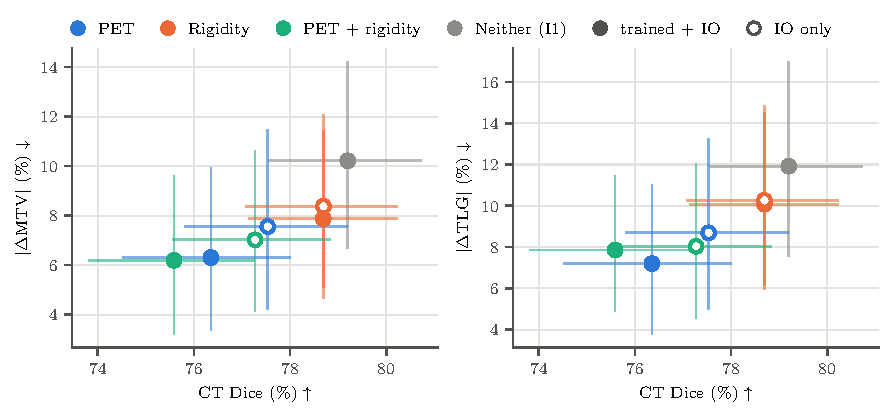
\includegraphics[width=\textwidth]{figures/q2.pdf}
\caption{Effect of the PET-preservation and rigidity losses and of where they act on the test set (CT Dice: 28 patients, 38 pairs; metabolic tumor volume [MTV] and total lesion glycolysis [TLG]: 26 patients, 30 pairs).
Color identifies the loss group; markers identify where the losses act (square: only in network training, shown before IO; filled circle: in training and IO; hollow circle: only in IO, on the network trained without losses).
Without losses: network output ($\times$) and with IO ($+$).
Lines connect configurations of the same loss group.
Each point is the mean over patients after averaging each patient's eligible pairs; uncertainty and significance tests are reported in Table~\ref{tab:ablations}.}
\label{fig:q2}
\end{figure}
